%! Author = robmandelings
%! Date = 02/12/2022

% Preamble
\documentclass[11pt]{article}

% Packages
\usepackage{amsmath}
\usepackage{float}
\usepackage{graphicx}
\usepackage[left=20mm, right=20mm]{geometry}
\usepackage{hyperref}

\hypersetup {
    colorlinks=true,
    linkcolor=blue,
    filecolor=magenta,
    urlcolor=cyan,
    pdftitle={Report},
    pdfpagemode=FullScreen,
}

id:4186629
id: 126

\bibliographystyle{plain}

\newcommand{\studentA}{Name: Rob Mandelings\\Student ID: 20193884\\}
\newcommand{\studentB}{Name: Jasper De Laet\\Student ID:20192214\\}

\title{Information Retrieval: Chess game retrieval based on board similarity}
\author{\studentA \\ \studentB}

% Document
\begin{document}
    \maketitle


    \section{Introduction}

    Learning and getting better at chess can be a difficult but satisfying process. As the field of artificial intelligence has grown substantially in the last couple of decades, so has the amount of AI based chess computers and solving systems. Often the reasoning behind the choices of such an AI based computer can be hard to explain and even harder to learn from, because such a system does not `think' the way a human chess player does.

    In this project we try a different way for creating an informative and educational chess system. As there are an enormous amount of chess games played already and still being played everyday, we used an information retrieval based approach. The objective is to retrieve games based on the similarity between the board positions in these already played games and a given chess board position. This would allow a user to analyse already played games more quickly and to improve his strategy for certain situations.


    \section{Problem Definition}

    Chess is a very popular board game between two players, where each player has a corresponding color. When the game starts, each player starts with an equal number of pieces, with each piece of a certain type. Every type of piece has different rules that govern which locations it may move to. If a reachable square is already occupied by a piece of the opposite side, this piece is allowed to move to that square. In this case, the piece of the opponent gets removed from the board. The goal is to place the king of the opponent into a checkmate position, i.e.\ the king is under immediate attack and cannot move to a position where it will not be attacked.

    At each step, a player has the option to move a single piece on the board, possibly removing a piece of the opposite color.

    As there are many ways in which to play game, people might wonder what might be a good move, given a particular board configuration. Therefore, it might be useful to look at similar board configurations for games that have been played in history in order to see what other people did in a similar setting as well as how the game ended. This makes it easier to perform analysis on board configurations and decide what is a good tactic or not.

    After the introduction and motivation for the project, we will now formulate our problem statement. The goal is to retrieve a relevant list of games (documents) which is sorted in a certain decreasing order. This order would be based on the similarity of a given board configuration (the query) and the board configurations in the games. So the more similar a board configuration inside a game to the given query, the higher this game would come up in the list.

    % TODO numskip
    % TODO complete games filtering
    % TODO check booster


    \section{Board Encoding}

    In order to create an efficient information retrieval system over chess games, we need to develop appropriate indexing for the documents. Therefore, we have to find a way to encode a board configuration so that the important information is preserved. We have used several encoding techniques, each of which highlights different features of a specific board configuration. The board state, reachability, attack, defense and ray-attack are based on the ideas and closures of \cite{SimilarChessPositions}. For a more mathematical explaination we refer to this as well.

    \subsection{Board State}

    The first encoding is the most straightforward, where each piece on the board is encoded. Every piece encoding consists of a piece type, color and position on the board. An example can be seen on (placeholder)

    If the board state query is enabled

    \subsection{Reachability}

    This encoding converts the board state into a list of reachable squares, for every piece on the board. A reachable square for a piece is considered to be a square where this piece is allowed to move to on its turn according to the rules of the game. Board positions that have reachabilities similar to the query board position is regarded as a better match.

    Another idea included in the reachability is the distance between the piece and the reachable square. The larger the distance, the smaller the weight that is given to this reachable square. An example is given on figure (figure).
    The weight $w$ is computed as follow:\\

    $w = 1 - \dfrac{7 * d((x,y),(x',y'))}{64}$ \\

    Here coordinate $(x,y)$ corresponds to the square of a particular piece, and $(x',y')$ to a reachable square. The distance function used is the Chebychev distance.\\

    \subsection{Attack}

    Another encoding is attack, where the board is converted into a sequence of squares with opponents that can be attack by another piece. This encoding is performed for each piece on the board, and concatenated as a single string. You can see an example of this on figure ()

    \subsection{Defense}

    This is similar to the attack encoding, except that the squares should now contain pieces of the same color. Thus, each piece that `attacks' a piece of its own color, actually defends it, as the defended pieces cannot be taken without risk. An example is given at figure ().

    \subsection{Ray-Attack}

    Ray-Attack is a more generalized form of the Attack encoding, where not only direct attack squares are considered, but also the attack squares that go through other pieces. Boards that have similar ray-attacks can be considered more similar than those who do not, as the ray-attacked pieces may become vulnerable if one of the directly attacked pieces move.

    \subsection{Check}

    A simple, yet powerful encoding we have implemented is Check. It is apparent to see that boards in a similar check state should be much more relevant to each other than other boards, mainly because being checked limits the moves that you can make. In case the board is in the check state, the color that is being checked as well as the pieces that attack the king are encoded. These terms make sure that the check similarity between boards goes up if the same color is being check, and is maximal if the pieces that attack the king are also equal. For example, the board that is used as query has a black queen that attacks the white king (figure todo).

    Board, Reachability, Attack, Defense
    check:black;check:white

    \subsection{Other possibilities}

    We have only implemented a sample of the possible encodings for these board configurations, as there is other useful information that might be encoded from these boards to get even more relevancy.

    % TODO er zou in principe ook met de parameters kunnen worden gespeeld om sommige encoderingen een groter gewicht / belang te laten hebben dan anderen om de relevancy te verhogen (bijvoorbeeld check of checkmate).


    \section{Document format}\label{sec:documentformat}

    % TODO full document format example include here

    This section explains the complete document format as well as provides an example of a single document containing all the board encodings as well as the game to which the board belongs. We have purposely split up the encodings into several fields instead of a single ``board\_encoding'' field, to allow for modularity. As you will see, it will be easy to toggle some of the encoding methods while querying for results in our user interface.

    Each of the encoding methods explained before encode the pieces in similarly. A single piece along its position on the board is regarded as a term that will be used for indexing, where the full encoding is a string consisting of a sequence of these terms. The only difference is that the reachability encoding also includes a weight for each piece.


    \section{Solr}

    In order to store and retrieve our documents, we used Solr, an application that uses Lucene under the hood. The reason we chose to use Solr instead of Lucene is that it is less difficult to set up, as Lucene is a library whereas Solr works out of the box.

    \subsection{BM25}

    The retrieval of our documents were performed with the algorithm Okapi BM25. The reason that we used this algorithm is that this enables ranked retrieval of documents, mainly because it allows boards to be retrieved in decreasing order of similarity. For this we used the parameters $k1 = 2.0$ and $b = 0.75$. Another key property of this algorithm is that it uses a bag-of-words function, for which the grammar and word order is disregarded. This makes sense, as the position of the pieces is already included in the encodings, therefore matching a piece at a position can be done regardless of the order.

    % TODO explain inverse document frequency

    There may be alternatives to the BM25 algorithm for our document retrieval which may perform better for this information retrieval project. However, the analysis of this part goes beyond the scope of the project.


    % TODO why did we use BM25 and not BM25F for example?
    % TODO Inverse Document Frequency (IDF) is a weight indicating how commonly a word is used. The more frequent its usage across documents, the lower its score.


    \section{Indexing}


    \section{Results}


    \section{Evaluation}

    It is hard to evaluate this information retrieval in an absolute manner, as the relevancy of the search results is hard to measure. If we had the time, we would ask chess players to rate the relevancy of the search results based on a set of predetermined chess positions. This information would subsequently be used to judge the relevance of the retrieval system. However, we are able to evaluate our retrieval system based on the difference between the relative similarity of the results, given a query. This evaluation is based on what we consider to be important similarities between chess boards. Such as the presence of a check, attack and defense positions, exact matches etc.

    First we will evaluate the search results based on exact matching. This means that if we query for a board configuration, and this exact board configuration is also present as a document in the index, it should be retrieved as the top result. We have provided a few figures () that demonstrate this functionality.

    \begin{figure}[H]
        \centering
        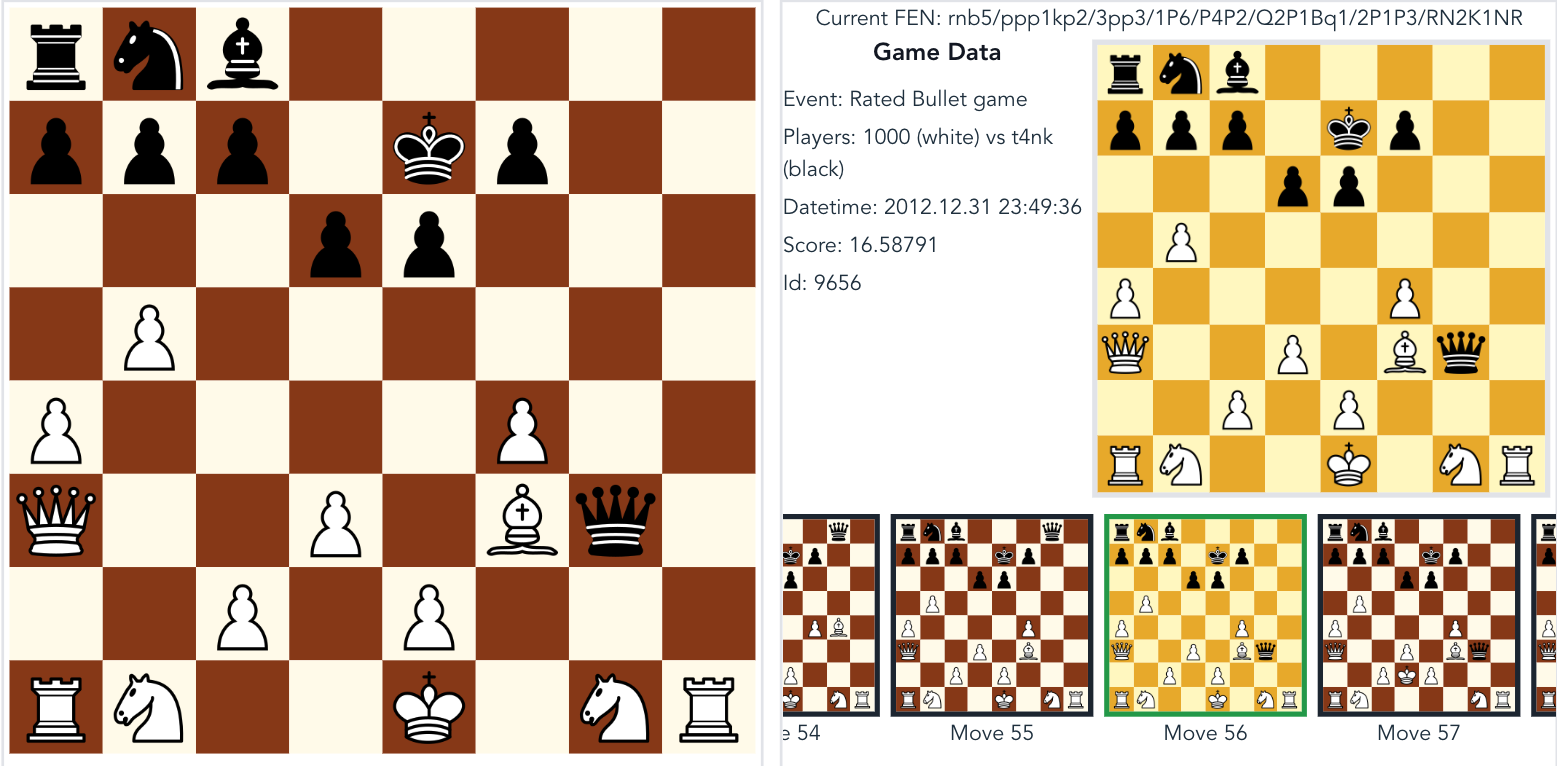
\includegraphics[width=14cm]{images/ExactMatch1-Bo}
        \caption{Exact matching; Only board similarity enabled.}
        \label{fig:ExactMatch1-Bo}
    \end{figure}

    We will now consider the attack and defense encodings to evaluate our retrieval system. The first

    Knight attacks bishop on g5, rook attacks bishop at g5, knight attack pawn at e5, white bishop attacks bishop at 5g (attach eachother).
    Pawn not defended at b4, bishop is defdedd by rook, king was not defended by the rook

    \begin{figure}[H]
        \centering
        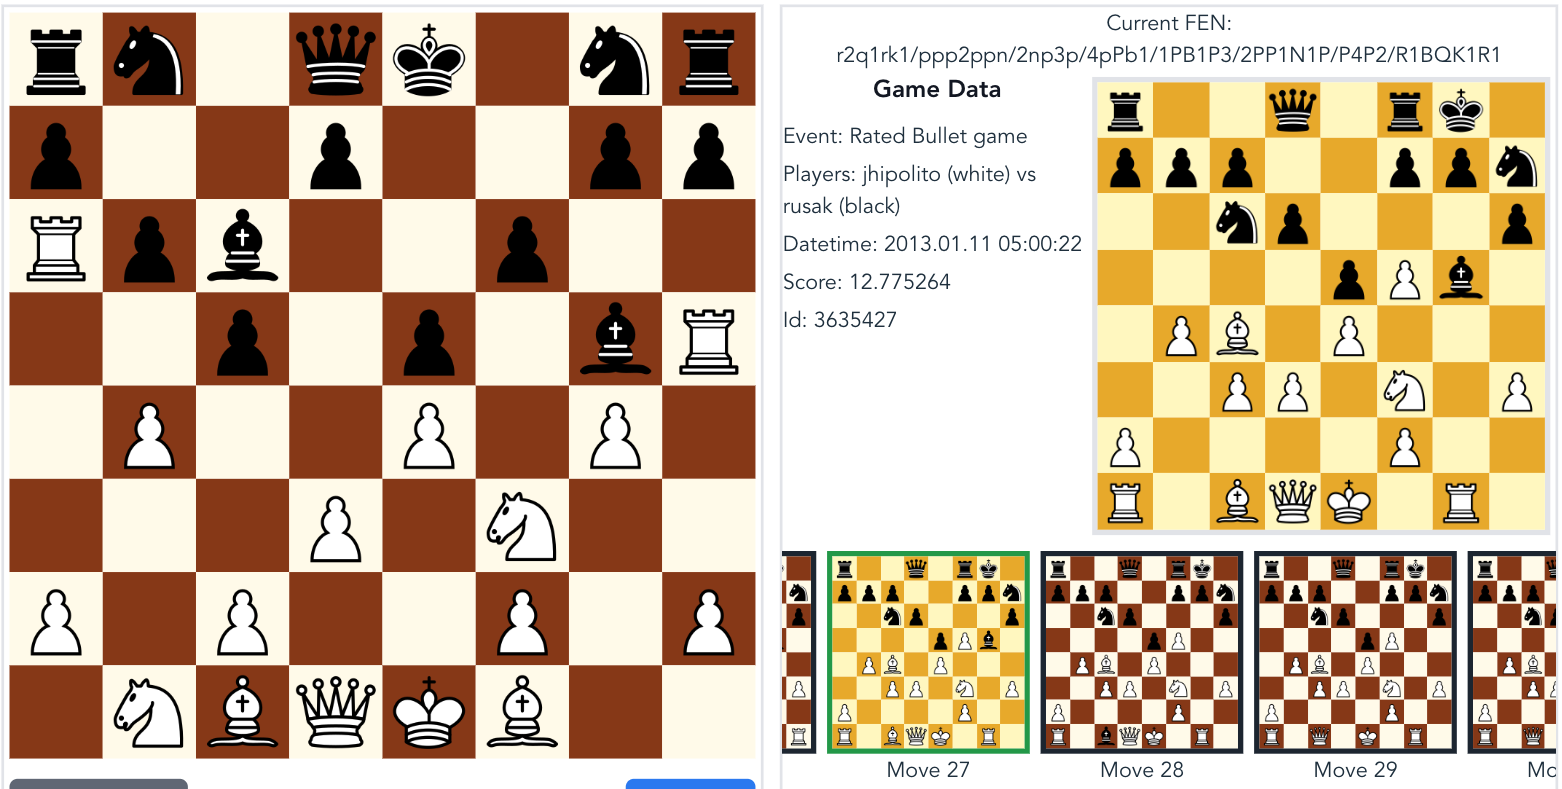
\includegraphics[width=14cm]{images/Attack}
        \caption{Top result for board query. Only attack similarity enabled.}
        \label{fig:Attack}
    \end{figure}

    For defense: rook defense pawn at a2, knight keeps defending c6, knight defends f7
    Two bishops attack each other in the query board, however in the result board they do not exist anymore. In the previous example, we could see these bishops were preserved. This implies that attack has a

    \begin{figure}[H]
        \centering
        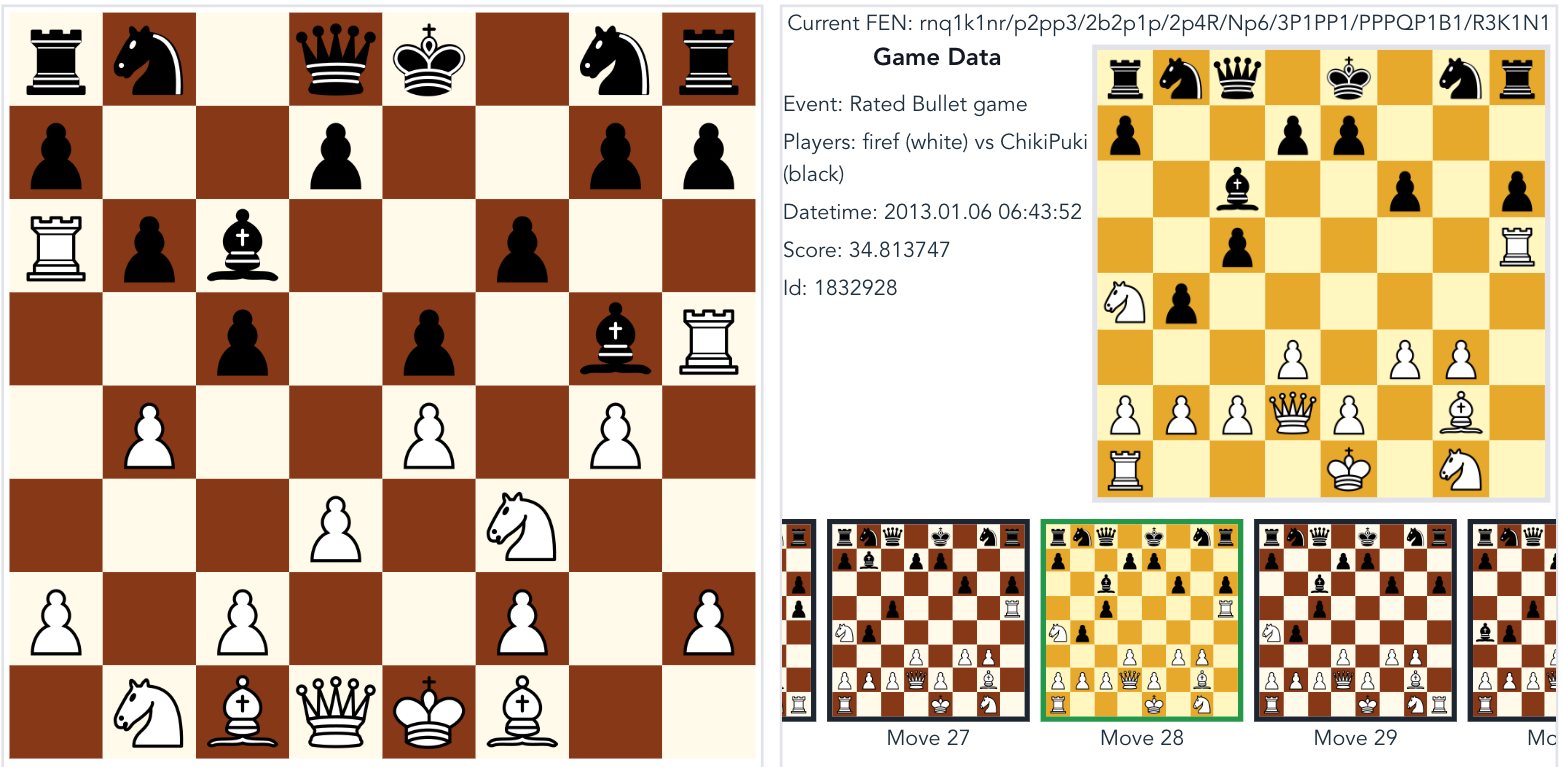
\includegraphics[width=14cm]{images/Defense}
        \caption{Top result for board query. Only defense similarity enabled.}
        \label{fig:Defense}
    \end{figure}

    Next, we will evaluate our check similarity. The board configuration we used as the query has a black king that is currently being checked by a white queen (figure ~\ref{fig:BlackCheckQuery}). Therefore a user might be interested in board games that also have a black king that is being attacked. The reason the top results should be boards that are also in the same situation with the black king, is that the moves for black are limited.

    \begin{figure}[H]
        \centering
        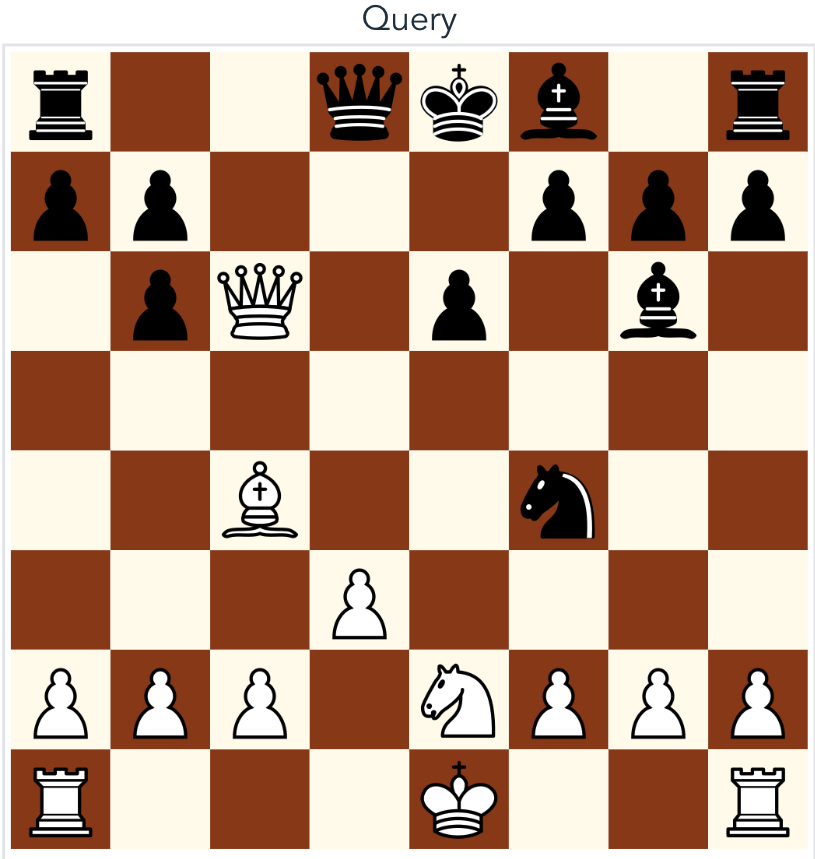
\includegraphics[width=8cm]{images/QueryBlackCheck}
        \caption{Query that is used to evaluate check}
        \label{fig:BlackCheckQuery}
    \end{figure}

    We will first analyse two top results for the query where only the board similarity is enabled. By comparing figures ~\ref{fig:BlackCheck1-Bo} and ~\ref{fig:BlackCheck2-Bo}, It is visible that the result where the black king is attacked has a slightly higher score than the result at figure ~\ref{fig:BlackCheck2-Bo}. This can be explained by the fact that the locations of some chess pieces in the results are identical to the query. It can also be observed that the black king being attacked does not yield a significant difference in score, which we will further examine in the next example.

    \begin{figure}[H]
        \centering
        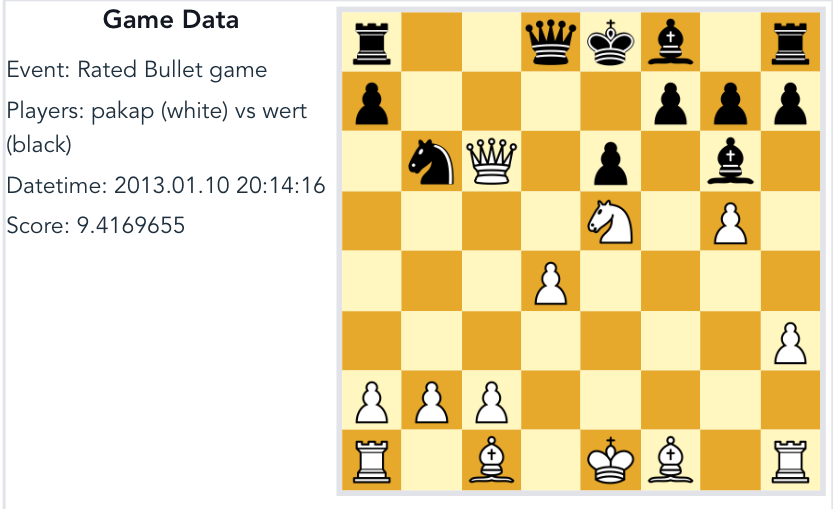
\includegraphics[width=14cm]{images/BlackCheck1-Bo}
        \caption{Query that is used to evaluate check}
        \label{fig:BlackCheck1-Bo}
    \end{figure}

    \begin{figure}[H]
        \centering
        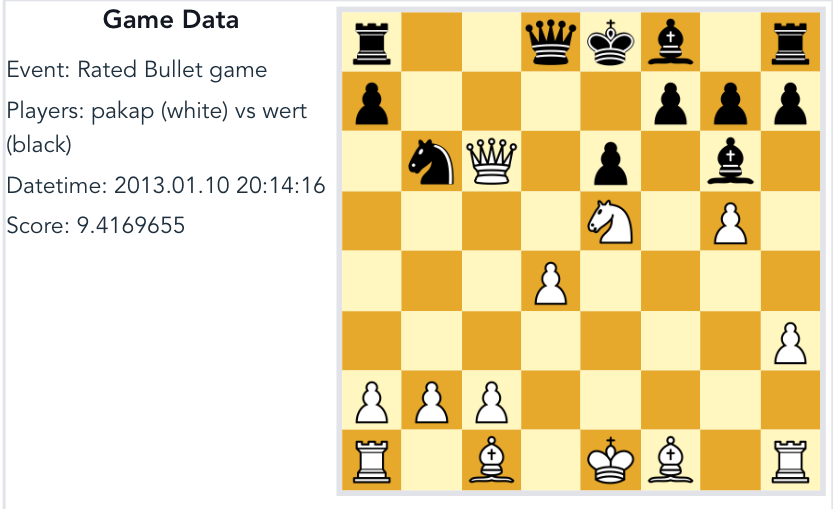
\includegraphics[width=14cm]{images/BlackCheck1-Bo}
        \caption{Query that is used to evaluate check}
        \label{fig:BlackCheck2-Bo}
    \end{figure}

    In this scenario (figures ~\ref{fig:BlackCheck1-BoReAtDe} and ~\ref{fig:BlackCheck2-BoReAtDe}), we have enabled the similarities Board, Reachability, Attack, Defense and RayAttack, except for Check. This way we can analyse the effect that Check similarity has on the obtained results. Figure ~\ref{fig:BlackCheck1-BoReAtDe} shows the result with the highest score, whereas figure ~\ref{fig:BlackCheck2-BoReAtDe} shows the second-best result. The black king is not being attacked in the board with the highest score, but is being attacked in the result with a slightly lower score, even though we find the result at ~\ref{fig:BlackCheck1-BoReAtDe} a more similar board configuration.

    \begin{figure}[H]
        \centering
        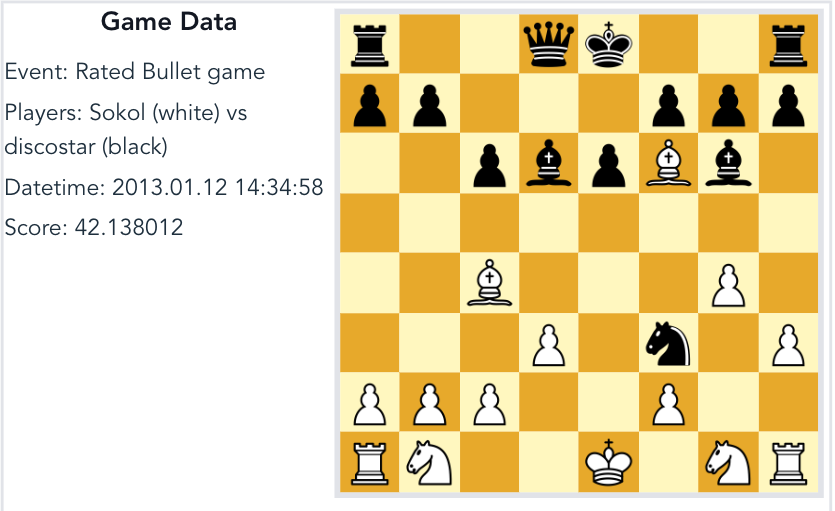
\includegraphics[width=14cm]{images/BlackCheck1-BoReAtDe}
        \caption{Query that is used to evaluate check}
        \label{fig:BlackCheck1-BoReAtDe}
    \end{figure}

    \begin{figure}[H]
        \centering
        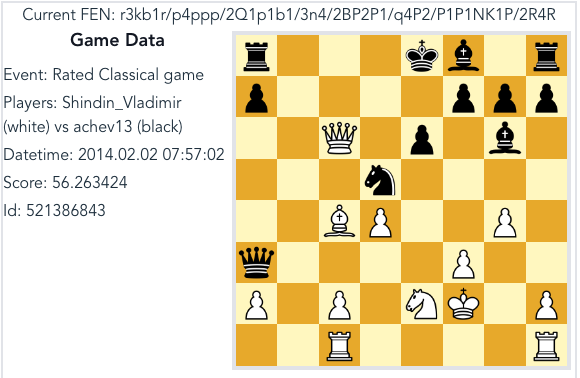
\includegraphics[width=14cm]{images/BlackCheck2-BoReAtDe}
        \caption{Query that is used to evaluate check}
        \label{fig:BlackCheck2-BoReAtDe}
    \end{figure}

    We will now enable all similarities, including Check. We can now see that the board with the highest score (\ref{fig:BlackCheck1-BoReAtDeCh}) has an attacked king, whereas the board with a lo

    \begin{figure}[H]
        \centering
        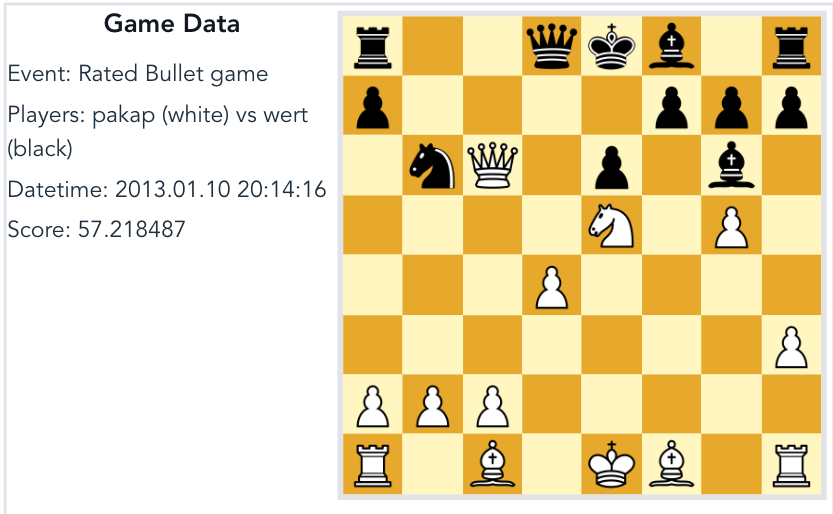
\includegraphics[width=14cm]{images/BlackCheck1-BoReAtDeCh}
        \caption{Query that is used to evaluate check}
        \label{fig:BlackCheck1-BoReAtDeCh}
    \end{figure}

    \begin{figure}[H]
        \centering
        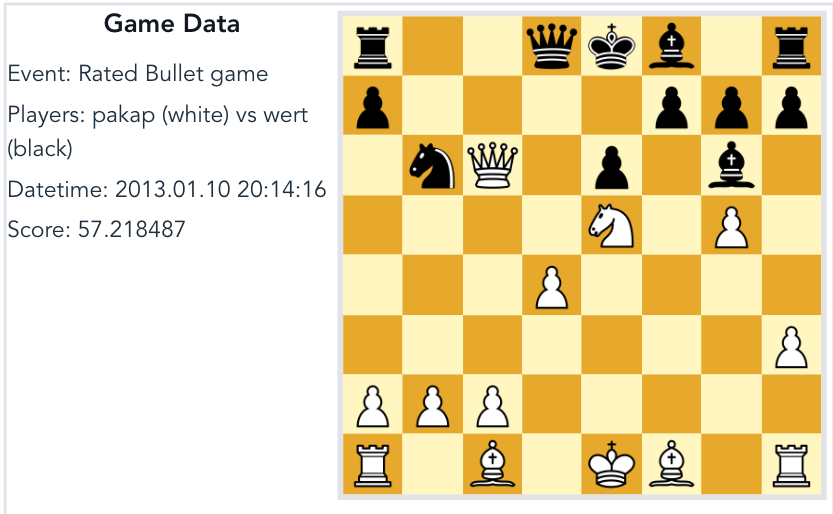
\includegraphics[width=14cm]{images/BlackCheck1-BoReAtDeCh}
        \caption{Query that is used to evaluate check}
        \label{fig:BlackCheck2-BoReAtDeCh}
    \end{figure}


    \section{Relevancy}

    % TODO can be hard to evaluate the relevance, if we would elaborate on this project even more, we would have users judge the relevance of chess board retrievals

    % TODO if there are boards that are exactly the same as the query, these should be retrieved and visible at the top (one evaluation)


    \section{User Interface}

    For demonstration purposes and ease of evaluation, we have created a user interface to run the queries and retrieve the results. A board configuration can be loaded by using an FEN configuration, either entering one manually or selecting a preset from the list. You can also turn on or off certain similarity encodings as you like, which is possible due to the usage of fields (section ~\ref{sec:documentformat}). After you have constructed the query (board configuration) and selected the desired encodings to be assist in the query, you can click on the search button to retrieve the results.

    After the query is performed, you will get a list of games sorted on relevancy, with the most relevant game at the top. You will also noticed that one board is highlighted that means this board configuration had the highest matching score and thus resulted in the retrieval of the corresponding game. All other boards of the game are also retrieved to see which moves led to the highlighted board configuration or what moves come next.

    As a side-note, a working demo of our project can be found at \href{http://chess.minetronic.com}{chess.minetronic.com}.


    \section{Suggestions}

    In this section we give some of the possible improvements that could be made to the system.

    An improvement that could be added is the rated-based filtering of the retrieval results. This would make the final results more relevant because games with a higher rating give more useful information.


    \section{Technologies}

    For the backend implementation of the project we mainly used Python. We chose Python as it was the most easy and readable programming language for us to work with and we did not want to lose time on learning other languages. To help us work with chess games and boards we used the chess library python-chess \cite{python-chess}. We used this library as it seemed useless to implement all the chess logic ourselves as this is not the purpose of our project. The library also contained a parser for both the PGN and FEN formats.

    \bibliography{refs}

% TODO possible question for the presentation: why encode the board in the current way instead of FEN?
\end{document}

